\newmdtheoremenv{ex}{Example}

\chapter{Knowledge-base Agnostic, Multilingual Entity Linking}
\graffito{
This chapter presents AGDISTIS, a novel approach towards graph-based, knowledge base-agnostic entity linking using Linked Data which won the ISWC Best Research Paper Award in 2014. 
AGDISTIS' has been published in~\cite{agdistis_ecai, agdistis_iswc,agdistisdemo}.
The author of this thesis implemented and co-evaluated AGDISTIS as well as its demo. 
Furthermore, he is the main author of the above mentioned publications. 
} 	
\label{cha:agdistis}

The Web in its current form is made up of at least 4,73  billion indexed Web pages.\footnote{Data gathered from \url{http://www.worldwidewebsize.com/} on October 25th, 2015.}
%One of the key steps towards extracting \ac{RDF} from text is the disambiguation of named entities.
%While several approaches aim to tackle this problem, they still achieve poor accuracy. 
%The vision behind the Web of Data is to provide a new machine-readable layer to the Web where the content of Web pages is annotated with structured data (e.g., \ac{RDF}a~\cite{\ac{RDF}a}).
%Most of these websites are unstructured in nature.
Thus, realizing the vision of a usable and up-to-date Web of Data requires scalable and accurate \ac{NLP} approaches that allow extracting \ac{RDF} from  unstructured data.
Three tasks play a central role when extracting \ac{RDF} from unstructured data:  \ac{NER}, \ac{NED}, also known as \ac{EL}~\cite{Mihalcea:2007:WLD:1321440.1321475}, and \ac{RE}.

For the first sentence of the Example~\ref{ex:obama}, a high-quality \ac{NER} approach would return the strings \texttt{Barack Obama} and \texttt{Washington, D.C.}.
An accurate \ac{NED} approach would use these already recognized named entities and map the strings \texttt{Barack Obama} resp. \texttt{Washington, D.C.} to \texttt{dbr:Barack\_Obama} and \texttt{dbr:Washington,\_D.C.} which are DBpedia~\cite{dbpedia-swj} resources. 
Furthermore, any \ac{RE} approach will extract the relation \texttt{wife} and output \texttt{dbr:Barack\_Obama dbo:spouse dbr:Michelle\_Obama} as RDF triple.
\begin{ex}
Barack Obama arrived this afternoon in Washington, D.C.. President Obama's wife Michelle accompanied him.
\label{ex:obama}
\end{ex}
While \ac{NER} has been explored extensively over the last decades~\cite{StanfordNER}, the disambiguation of named entities,\,i.e., the assignment of a resource's URI from an existing \ac{KB} to a string that was detected to label an entity, remains a difficult task.

\todo[inline]{@Me: Verbinde das mit dem vorherigen Kapitel}
Current \ac{NED} approaches suffer from three major drawbacks:
First, they poorly perform on Web documents~\cite{RatinovRo09}.
This is due to Web documents containing resources from different domains within a narrow context.
An accurate processing of Web data has yet been shown to be paramount for the implementation of the Web of Data~\cite{GER+13}.
%, Web data is a very worthwhile source of latest information which is often not yet captured in any knowledge base. 

Second, well-know approaches such as \emph{Spotlight}~\cite{spotlight} and \emph{TagMe 2}~\cite{TagMe2} have been designed to work on a particular \ac{KB}.
However, Web data contains resources from many different domains.
%Ttha named entity disambiguation framework has to be able to work on any knowledge base in order to capture content from different domains.
Hence, we argue that \ac{NED} approaches have to be designed in such a way that they are agnostic of the underlying \ac{KB}.

%Being capable of using specialized or language-specific knowledge bases should lead to high F-measures. 
Third, most state-of-the-art approaches rely on exhaustive data mining methods~\cite{Cucerzan07,rat:rot} or algorithms with non-polynomial time complexity~\cite{Kleb11WIMS}.
However, given the large number of entities that must be disambiguated when processing Web documents, scalable \ac{NED} approaches are of central importance to realize the Semantic Web vision.
%\todo[inline]{Micha: The sentence "Hence, we argue that \ac{NED}..." is not really good. From my point of View it sounds like "A \ac{NED}-algorithm has to use more than one \ac{KB} at the same time".}


We address this drawback by presenting AGDISTIS,  a novel \ac{NED} approach. Our contributions are as follows:
\begin{itemize}
\item We present AGDISTIS, a knowledge-base-agnostic approach for named entity disambiguation.
\item Our approach combines the \ac{HITS} algorithm with label expansion strategies and string similarity measures.
Based on this combination, AGDISTIS can efficiently detect the correct URIs for a given set of named entities within an input text. 
\item We show that our approach has a quadratic time complexity. Thus, it scales well enough to be used even on large knowledge bases (English, German and Chinese DBpedia, YAGO2 \ac{KB}~\cite{Yago2}).
\item We evaluate our approach on nine \emph{well-known and diverse open-source datasets} and four different knowledge bases as well as against four state-of-the-art named entity disambiguation frameworks.
Our results indicate that we outperform the state-of-the-art approach by up to $29\%$ F-measure.
\item AGDISTIS' demo is presented and deployed on three different languages (English, German and Chinese) and three different knowledge bases (DBpedia, the German DBpedia and the Chinese DBpedia) as well as tested against the YAGO2 \ac{KB}.
To the best of our knowledge, we therewith provide the first Chinese instantiation of entity linking to DBpedia.
\item We will also demonstrate the AGDISTIS web services endpoints for German, English and Chinese disambiguation and show how data can be sent to the endpoints.
%(1) We present AGDISTIS, an accurate and scalable framework for disambiguating named entities that is agnostic to the underlying knowledge base (KB) and show that we are able to outperform the state of the art by up to $29\%$ F-measure on these datasets.
%\todo[inline]{description of datasets? multilingual, multi-domain}
%We show the results of the framework on texts pertaining to manifold domains including news, sports, automobiles and e-commerce.
%In the following, we present the two ways of approaching AGDISTIS, architecture and workflow.
%One key step towards extracting structured data from unstructured data sources is the disambiguation of entities.
%With AGDISTIS, we provide a time-efficient, state-of-the-art, knowledge-base-agnostic and multilingual framework for the disambiguation of \ac{RDF} resources.
%Moreover, we present an extension based on topic modeling which improves the quality of the extraction in difficult cases by up to $3\%$.
\end{itemize}


The rest of this chapter is organized as follows: 
%First, a brief overview of related work is presented in Section~\ref{sec:relatedwork}.
We introduce the AGDISTIS approach in Section~\ref{sec:approach} and evaluate it in Section~\ref{sec:eval} against state-of-the-art tools, nine diverse datasets, four knowledge bases and three languages. 
%\todo{surface form richtig erklärt?}
%We analyze the contribution of certain properties to our disambiguation approach in the same section. 
%We conclude in Section~\ref{sec:conclusion} by highlighting research questions that emerged from this work.
Further data, detailed experimental results and source code for this paper is publicly available on our project homepage \url{http://aksw.org/Projects/AGDISTIS}.

\section{The AGDISTIS Approach} 
\label{sec:approach}

In this section, we formalize the task of \ac{NED}, present the architecture of AGDISTIS and highlight the candidate detection and their optimal assignment. 

\subsection{Named Entity Disambiguation}
\label{sec:ned}

The goal of AGDISTIS is to detect correct resources from a \ac{KB} $K$ for a vector $N$ of $n$ a-priori determined named entities $N_1,\ldots,N_n$ extracted from a certain input text $T$.
In general, several resources from a given knowledge base $K$ can be considered as candidate resources for a given entity $N_i$.
For the sake of simplicity and without loss of generality, we will assume that each of the entities can be mapped to $m$ distinct candidate resources.
Let $C$ be the matrix which contains all candidate-entity mappings for a given set of entities.
The entry $C_{ij}$ stands for the $j^{th}$ candidate resource for the $i^{th}$ named entity. 
Let $\mu$ be a family of functions which maps each entity $N_i$ to exactly one candidate $C_{ij}$. 
We call such functions \emph{assignments}.
The output of an assignment is a vector of resources of length $|N|$ that is such that the $i^{th}$ entry of the vector maps with $N_i$.

Let $\psi$ be a function which computes the similarity between an assignment $\mu(C,N)$ and the vector of named entities $N$.
The \emph{coherence} function $\phi$ calculates the similarity of the knowledge base $K$ and an assignment $\mu$, cf. Ratinov et al.~\cite{rat:rot}, to ensure the topical consistency of $\mu$.
The coherence function $\phi$ is implemented by the  \ac{HITS} algorithm, which calculates the most pertinent entities while the similarity function $\psi$ is,\,e.g., string similarity.
Given this formal model, the goal is to find the assignment $\mu^\star$ with
\begin{equation*}
\mu^\star= \operatorname*{arg\,max}\limits_{\mu}\left(\psi(\mu(C,N), N) + \phi(\mu(C,N),K)\right).
\end{equation*}

The formulation of the problem given above has been proven to be NP-hard, cf. Cucerzan et al.~\cite{Cucerzan07}.
Thus, for the sake of scalability, AGDISTIS computes an approximation $\mu^{+}$ by using  \ac{HITS}, a fast graph algorithm which runs with an upper bound of $\Theta(k\cdot |V|^2)$ with $k$ the number of iterations and $|V|$ the number of nodes in the graph.
Furthermore, using \ac{HITS} leverages 1) scalability, 2) well-researched behaviour and 3) the ability to explicate semantic authority~\cite{HITS}. 

\subsection{Architecture}
\begin{figure*}[h!tb]
\centering
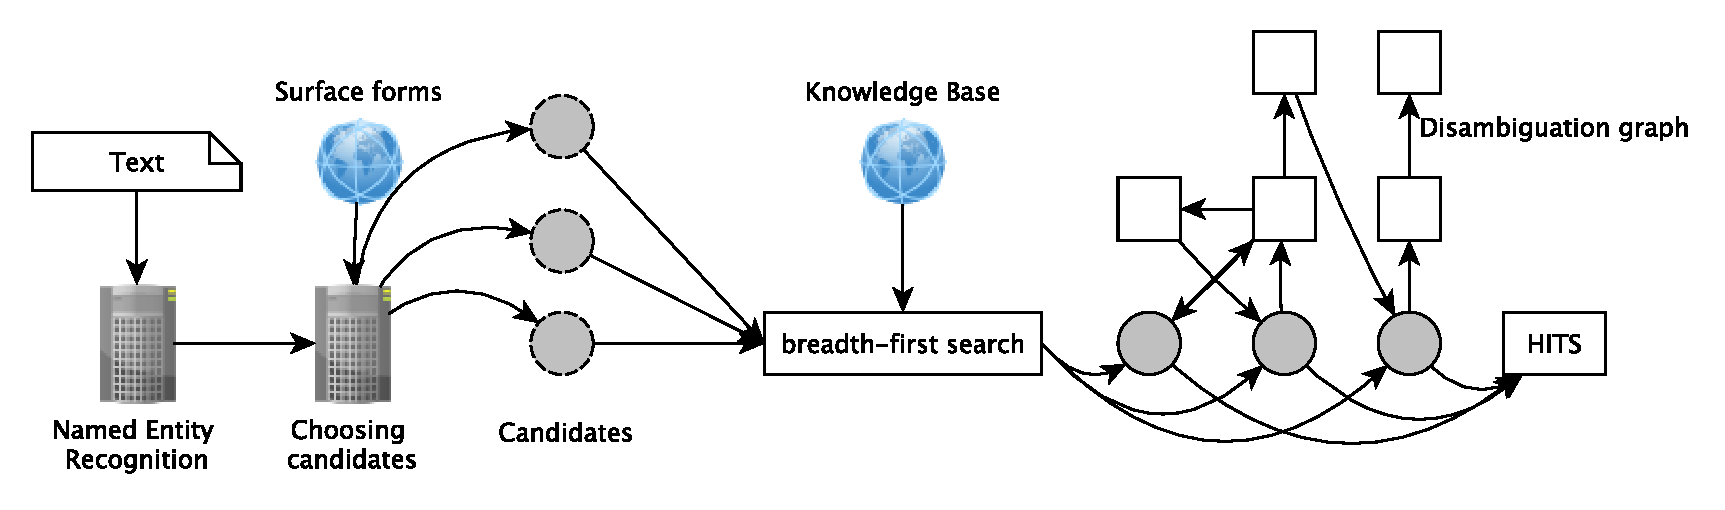
\includegraphics[width=\linewidth]{part_02/unstructured_annotation/fig/overview.pdf}
\caption{Overview of AGDISTIS.}
\label{fig:overview_agdistis}
\end{figure*}

Our approach to \ac{NED} thus consists of three main phases as depicted in Figure~\ref{fig:overview_agdistis}.
Given an input text $T$ and a named entity recognition function, e.g., FOX~\cite{FOX}, we begin by retrieving all named entities from the input text.
Thereafter, we aim to detect candidates for each of the detected named entities.
To this end, we apply several heuristics and make use of known surface forms~\cite{spotlight} for resources from the underlying \ac{KB}.
The set of candidates generated by the first step is used to generate a disambiguation graph. 
Here, we rely on a graph search algorithm which retrieves context information from the underlying \ac{KB}. 
Finally, we employ the  \ac{HITS} algorithm to the context graph to find authoritative candidates for the discovered named entities.
We assume that the resources with the highest authority values represent the correct candidates.
All algorithms in AGDISTIS have a polynomial time complexity, leading to AGDISTIS also being polynomial in time complexity.
Choosing candidates relates to the notion of $\phi$ while calculating the authority values confers to $\psi$.
In the following, we present each of the steps of AGDISTIS in more detail.

\subsection{Candidate Detection}\label{choosing}

In order to find the correct disambiguation for a certain set of named entities, we first need to detect candidate resources in the \ac{KB}. 
We begin by creating an index comprising all labels of each resource.
Our approach can be configured to use any set of properties as labeling properties, e.g., those in Ell et al.~\cite{ELL+11}. 
For our experiments, we only considered \texttt{rdfs:label} as labeling property.
In addition, our approach can make use of known \emph{surface forms} for each of the resources in case such knowledge is available~\cite{spotlight}.
These are simply strings that are used on the Web to refer to given resources.
Surface forms are simply added to the set of available labels for each resource, cf.\ Section~\ref{eval}.
In this paper, we do not consider abbreviations although these could be easily regarded by adding further labels into the \ac{KB}, e.g., via WordNet~\cite{wordnet}.
%\todo[inline]{remove the above sentence because of missing scientific eval?}

Next to searching the index, we apply a \emph{string normalization} approach and an \emph{expansion policy} to the input text:

The string normalization is based on eliminating plural and genitive forms, removing common affixes such as postfixes for enterprise labels and ignoring candidates with time information (years, dates, etc.) within their label.
For example, the genitive \texttt{New York's} is transformed into \texttt{New York}, the postfix of \texttt{Microsoft Ltd.} is reduced to \texttt{Microsoft} and the time information of \texttt{London 2013} is ignored.

Our \emph{expansion policy} is a time-efficient approach to coreference resolution, which plays a central role when dealing with text from the Web, cf.~Singh et al.~\cite{singh}. 
In web and news documents, named entities are commonly mentioned in their full length the first time they appear, while the subsequent mentions only consist of a substring of the original mention due to the brevity of most news data.
For example, a text mentioning Barack Obama's arrival in Washington D.C. will commonly contain \texttt{Barack Obama} in the first mention of the entity and use strings such as \texttt{Obama} or \texttt{Barack} later in the same text, see Example~\ref{ex:obama}.
We implement this insight by mapping each named entity label, e.g., \texttt{Obama}, which is a substring of another named entity label that was recognized previously, e.g., \texttt{Barack Obama}, to the same resource, i.e., \texttt{dbr:Barack\_Obama}.
If there are several possible expansions, we choose the shortest as a fast coreference resolution heuristic for web documents.
Without the expansion policy AGDISTIS suffers from a loss of accuracy of $\approx4\%$.

%This is simply due to humans readers being able to carry out a co-reference analysis on the fly.

%Internally, AGDISTIS begins its disambiguation by employing the string expansion policy\footnoterecall{myfootnote}.
%Our policy stores all named entity strings in order of their string length.
%If we recognize an entity string matching a part of an already processed entity, we expand the current string to the one stored earlier.
%This assumes both named entities mention the same instance.


%After expanding named entities we harness additional well-known linguistic heuristics.
%Named entities occur often in plural and genitive forms,\,i.e., AGDISTIS tries to identify and stem those words. 
%For example, the genitive form of the named entity \texttt{Obama's} is transformed into \texttt{Obama}.
%Additionally, AGDISTIS reduces plural strings such as \texttt{Obamas} to the singular form \texttt{Obama}.
%Another heuristic is to remove common affixes. 
%For example, we remove affixes which stands for the form of enterprises, such as \emph{corp} and \emph{ltd},\,e.g., \texttt{Hanover Insurance Corp.} is shrunk to \texttt{Hanover Insurance} in order to find candidates for this string in the \ac{KB}.  	
%We observed a significant data quality problem considering affixes in the examined knowledge bases.
%AGDISTIS also eliminates candidates with years and dates within the label so as to be time-independent and to prune the search space.
%One key advantage of Linked Data is the possibility to retrieve a class for each instance in a \ac{KB}.
%By using entity types (obtained via the \texttt{\ac{RDF}:type} property), a domain fitting of possible candidates is implemented, narrowing the search space. 
\begin{table}[htb!]
\centering
 \begin{tabular}{lll}
	\toprule
\textbf{} & \textbf{Class} & \texttt{\textbf{rdf:type}}\\
\midrule
DBpedia & Person & \texttt{dbo:Person}, \texttt{foaf:Person}\\
DBpedia & Organization & \texttt{dbo:Organization}, \texttt{dbo:WrittenWork} (e.g., Journals) \\
DBpedia & Place & \texttt{dbo:Place}, \texttt{yago:YagoGeoEntity} \\
\midrule
YAGO2 & Person & \texttt{yago:yagoLegalActor}  \\
YAGO2 & Organization & \texttt{yago:yagoLegalActor}, \\
  &   &  \texttt{yago:wordnet\_exchange\_111409538} (e.g., NASDAQ) \\
YAGO2 & Place & \texttt{yago:YagoGeoEntity} \\
\bottomrule

 \end{tabular}
  \caption{DBpedia  and YAGO2 classes used for disambiguation classes.}
  \label{tab:tableOfClasses}
 \end{table}
 
 
Additionally, AGDISTIS can be configured to fit named entities to certain domains to narrow the search space.
Since our goal is to disambiguate persons, organizations and places, AGDISTIS only allows candidates of the types mentioned in Table~\ref{tab:tableOfClasses} when run on DBpedia and YAGO2.
Adding general types will increase the number of candidates and thus decrease the performance.
Obviously, these classes can be altered by the user as required to fit his purposes. 




The resulting candidate detection approach is explicated in Algorithm~\ref{findingCandidates}.
%If a \ac{KB} provides redirect and disambiguation URLs, AGDISTIS can benefit from them.
%\todo[inline]{added  a virtual function in this algorithm 1 for the grammatical functions}
%For example, it is straightforward to use \texttt{dbo:wikiPageRedirects} for identifying multiple labels for one instance. 
%Of course AGDISTIS ignores disambiguation entities as they would not help accomplishing the disambiguation goal and finding $\mu^{+}$. 
%\todo[inline]{AN:What's a disambiguation entity?}
In its final step, our system compares the heuristically obtained label with the label extracted from the \ac{KB} by using \emph{trigram similarity} which is an n-gram similarity with $n=3$. 

\begin{algorithm}[htb!]
\KwData{label of a certain named entity $N_i$, $\sigma$ trigram similarity threshold}
\KwResult{$C$ candidates found}
$C \longleftarrow \emptyset$\;
{\bf label } $\longleftarrow$ {\bf normalize(label)}\;
{\bf label } $\longleftarrow$ {\bf expand(label)}\;
$ \displaystyle \bar C \longleftarrow$ {\bf searchIndex(label)}\;
\For{{\bf c} $\in \bar C$}{
    \If{$\neg${\bf c .matches([0-9]$^+$)}}{
        %\If{$\neg${\bf isDisambiguationSite(c})} {
         %          {\bf continue}\;
          %      }
        \If{{\bf trigramSimilarity(c, label)}$ \geq \sigma$}{
            \If{{\bf fitDomain(c)}} {
                $C \longleftarrow C \cup $ {\bf c}\;
            }
        }
        % The same as the two ifs above but with a continue
        %\If{{\bf trigramSimilarity(c, label)}$ < \sigma$} {
        %           {\bf continue}\;
        %        }
        %% {\bf c} $\longleftarrow$ {\bf redirect(c)}\;
        %\If{{\bf fitDomain(c)}} {
        %     $C \longleftarrow C \cup $ {\bf c}\;
        %        } 
        %}
    }
}
\caption{Searching candidates for a label.}
\label{findingCandidates}
\end{algorithm}

\subsection{Computation of Optimal Assignment}

Given a set of candidate nodes, we begin the computation of the optimal assignment by constructing a disambiguation graph $G_d$ with search depth $d$.
To this end, we regard the input \ac{KB} as a directed graph $G_K = (V, E)$ where the vertices $V$ are resources of $K$, the edges $E$ are properties of $K$ and $x,y\in V, (x,y) \in E \Leftrightarrow \exists p : (x, p, y) \mbox{ is an \ac{RDF} triple in }K$.
Given the set of candidates $C$, we begin by building an initial graph $G_0 = (V_0, E_0)$ where $V_0$ is the set of all resources in $C$ and $E_0=\emptyset$. %$\forall (x, y) \in V_0^2, (x, y) \in E_0 \Rightarrow (x, y) \in K$.
Starting with $G_0$ we extend the graph in a breadth-first search manner.
Therefore, we define the extension of a graph $G_i = (V_i, E_i)$ to a graph as follows:
\begin{equation}
\rho(G_i) = G_{i+1} = (V_{i+1}, E_{i+1}) \textnormal{ with } i=0, \ldots, d
\end{equation}
\begin{equation}
V_{i+1} = V_i \cup \{y : \exists x \in V_i \wedge (x, y) \in E\}
\end{equation}
\begin{equation}
E_{i+1} = \{(x,y) \in E: x, y \in V_{i+1}\}
\end{equation}
We iterate the $\rho$ operator $d$ times on the input graph $G_0$ to compute the initial disambiguation graph $G_d$.

%Empirically, we see no effect on the \mbox{F-measure} when using spread activation instead~\cite{Kleb11WIMS} (despite the obvious extra computational costs).

After constructing the disambiguation graph $G_d$, we need to identify the correct candidate node for a given named entity.
Using the graph-based  \ac{HITS} algorithm, we calculate authoritative values $x_a,y_a$ and hub values $x_h,y_h$ for all $x,y\in V_d$.
We initialize the authoritative and hub values $x_a$ respectively $x_h$:
\begin{equation}
\forall x \in V_d, x_a=x_h=\frac{1}{|V_d|}  .
\end{equation}
Afterwards, we iterate the equations $k$ times as follows: 
\begin{equation}
x_a = \sum_{(y,x)\in E_d} y_h
\end{equation}
\begin{equation}
y_h = \sum_{(y,x)\in E_d} x_a 
\end{equation}
We choose $k$ according to Kleinberg~\cite{HITS}, i.e., 20 iterations, which suffice to achieve convergence in general. %d authoritative values $x_a$ and hub values $y_h$.
Afterwards, we identify the most authoritative candidate $C_{ij}$ among the set of candidates $C_i$ as correct disambiguation for a given named entity $N_i$. %sort the nodes according to their authoritative values in descending order. 
%The first candidate for a certain named entity is assumed to be the correct disambiguation.
When using DBpedia as \ac{KB} and $C_{ij}$ is a redirect AGDISTIS uses the target resource. %follows redirecting resources transitively. %can use redirections to di%maps redirecting resources to their most authoritative redirection.
AGDISTIS' whole procedure is presented in Algorithm~\ref{algooverview}.
As can be seen, we calculate $\mu^{+}$ solely by using polynomial time complex algorithms.
%Thus, we observe on average better run time performance than the state-of-the-art approach AIDA, see Section~\ref{results}. % Appendix Figure 3).
%\todo[inline]{Again, we have no Appendix here}
\begin{algorithm}[htb!]
\KwData{$N=\{N_1,N_2\dots N_n\}$ named entities, $\sigma$ trigram similarity threshold, $d$ depth, $k$ number of iterations}
\KwResult{$C = \{C_1,C_2\dots C_n\}$ identified candidates for named entities}
$E \longleftarrow \emptyset$\;
$V \longleftarrow${\bf insertCandidates($N, \sigma$)}\;
$G \longleftarrow (V,E)$\;
$G \longleftarrow${\bf breadthFirstSearch($G,d$)}\;
{\bf  HITS($G(V,E), k$)}\;
{\bf sortAccordingToAuthorityValue(V)}\;
\For{$N_i \in N$} {
    \For{$v \in V$}{
        \If{$v$ {\bf is a candidate for} $N_i$  }{
              {\bf store($N_i$,$v$)}\;
              {\bf break}\;
          }
     }
}
\caption{Disambiguation Algorithm based on \ac{HITS} and Linked Data.}
\label{algooverview}
\end{algorithm}


For our example, the graph depicted in Figure~\ref{fig:example} shows an excerpt of the input graph for the  \ac{HITS} disambiguation algorithm when relying on DBpedia as \ac{KB}. 
%Depending on the used \ac{KB} properties may exist that lead to bi-directional edges (e.g., \texttt{sex} vs. \texttt{fatherOf}).
The results can be seen in Table~\ref{tab:example}. 
%Obviously a disambiguation towards the correct named entity URIs is possible.
%\todo{what happens if the \ac{KB} does not contain the correct entity, does the algorithm answer null, but is encompanied with closed world assumption, we know all entities we annotated}
%Since we assume a closed-world scenario our algorithm supposes every entity to be in the \ac{KB}.

\begin{figure}[htb!]
	\begin{minipage}[b]{0.57\textwidth} 
       % \begin{figure}
         \centering
        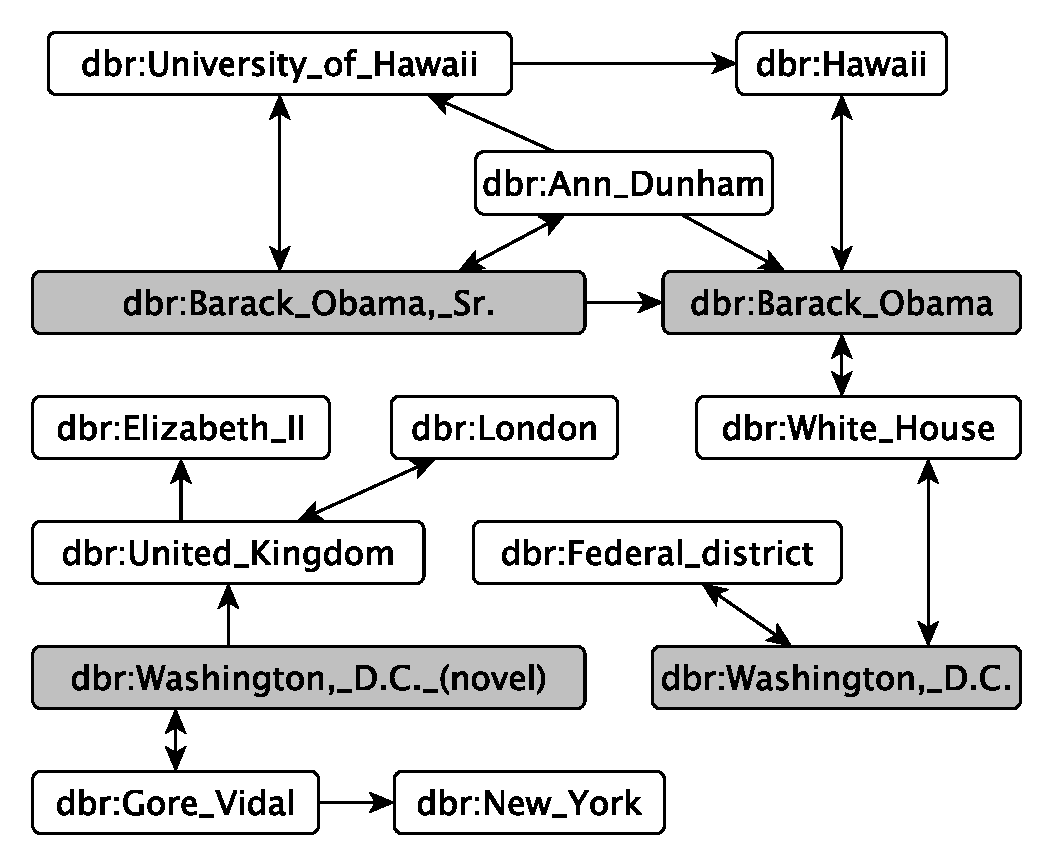
\includegraphics[width=\linewidth]{part_02/unstructured_annotation/fig/exampleGraph.pdf}
        \caption{One possible graph for the example sentence, with candidate nodes in grey.}
        \label{fig:example}
      %  \end{figure}
    \end{minipage}
	\hfill
	\begin{minipage}[b]{0.42\textwidth}
       % \begin{table}
        \centering
        
        \resizebox{\textwidth}{!}{ 
        \begin{tabular}{lc}
            \toprule
            \textbf{Node}  & \textbf{$x_a$} \\
            \midrule
            \texttt{dbr:Barack\_Obama} & 0.273 \\
            \texttt{dbr:Barack\_Obama,\_Sr.} & 0.089 \\
            \texttt{dbr:Washington,\_D.C.} & 0.093 \\
            \texttt{dbr:Washington,\_D.C.\_(novel)} & 0.000 \\
            \bottomrule
        \end{tabular}}
        \captionof{table}{Nodes and their according authority weights for the example graph.}
        \label{tab:example}
        \vspace{1.8cm}
       % \end{table}
	\end{minipage}
\end{figure}

%%Idea of the extension
%The most words of a document given to AGDISTIS are no named entities.
%Therefore, AGDISTIS does not use them in its workflow.
%Because a human reader would use all words for the disambiguation task we thought of an extension of AGDISTIS which uses the additional words, too.
%With these words AGDISTIS would be able to recognize the topical structure of the document and could use these information for the disambiguation task.
%Therefore, we added an extension which uses topic modeling to consider the topical structure.

%%what is topic modeling
%\emph{Probabilistic topic modeling} is a research area that aims to discover thematic information inside large corpora \cite{Blei:2012:PTM:2133806.2133826}.
%It is based on the definition of generative models that describe the creation of documents and how this process is influenced by latent topics.
%A very famous model is \emph{Latent Dirichlet Allocation (LDA)} \cite{Blei:2003:LDA:944919.944937}.
%Its generative process is based on a set of Topics $T$ and a vocabulary $V$.
%For the creation of a document $d$ the distribution of the topics inside this document $\theta_d=\left \{P(t_0|d), \ldots, P(t_{|T|}|d) \right \}$ is sampled.
%After that for every $i$th-word the id $z_i$ of a topic $t_{z_i}$ is sampled from $\theta_d$.
%Every topic $t \in T$ has a vector $\phi_{t}=\left \{P(w_0|t), \ldots, P(w_{|V|}|t) \right \}$ which defines the probabilities of all words under this topic.
%After $z_i$ has been sampled the word is sampled from $\phi_{t_{z_i}}$ \cite{Blei:2012:PTM:2133806.2133826}.
%Figure TODO shows the graphical model of LDA.
%The figure contains $\alpha$ and $\beta$ which are hyperparameter for the $\theta$ and $\phi$ distributions respectively.
%\todo[inline]{Add graphic with plate notation}

%In figure TODO all variables are white except the word $w$ which is shaded.
%This means that $w$ is the only variable which can be observed and all other variables are latent.
%So starting with the observable words inside of the documents of a corpus the other variables have to be inferenced.
%Because a direct solution of the inference problem is intractable there are several algorithms for approximating the variables \cite{Blei:2012:PTM:2133806.2133826}.
%For our experiments we used Mallet which contains an implementation of Gibbs-Sampling \cite{McCallumMALLET,griffiths2004finding}.

%\todo[inline]{* definition \newline* LDA \newline* generative model \newline* how do we use it \newline* where does the model come from\newline * \textbf{what are we doing with the model and the texts}}

\section{Evaluation}
\label{sec:eval}

This section is divided into four parts. 
First, we explain the experimental setup, i.e., which measures we chose for evaluation.
Then, we describe the datasets underlying the experiments. 
Afterwards, the evaluation results are analyzed and conclusion are drawn. 
We devote a single subsection to the generation and evaluation of the Chinese benchmark since it is the first benchmark w.r.t. Chinese \ac{NED}.

\subsection{Experimental Setup}
\label{eval}
The aim of our evaluation is two-fold.
First, we want  to determine the F-measure achieved by our approach on different datasets.
Several definitions of F-measure have been used in previous work on \ac{NED}.
Cornolti et al.~\cite{cornolti} define the micro F-measure (F1) w.r.t. a strong annotation match, i.e., a binary relation, and the possibility of assigning null to an entity.
This micro F-measure, which we use throughout our evaluation, aggregates all true/false positives/negatives over all documents.
\todo[inline]{Macro Fmeasure @ Micha?}
Thus, it accounts for larger contexts in documents with more annotations, cf. Cornolti et al.~\cite{cornolti, GERBIL}.
For a more detailed explanation of evaluation measures please cf. Chapter~\ref{cha:gerbil}.

%In addition to the traditional definition of false and true positives and negatives when given a reference mapping between strings and resources, 
%we regarded the assignment of a resource to a string as a \emph{false positive} if no resource from the \ac{KB} mapped with the string or if the string was assigned to the wrong resource.
%Furthermore, the assignment of a resource was considered a \emph{false negative} if the approach returned that no resource mapped the string although there was a resource in the \ac{KB} that did.

Second, we want to know how AGDISTIS performs in comparison to other state-of-the-art \ac{NED} approaches. 
Thus, we compare AGDISTIS with TagMe 2~\cite{TagMe2}, the best approach according to Cornolti et al.~\cite{cornolti} as well as with AIDA~\cite{AIDA} and DBpedia Spotlight~\cite{spotlight} because they are well-known in the Linked Data community. 
AGDISTIS is designed to be agnostic of the underlying \ac{KB}.
Thus, we use the German and English DBpedia \ac{KB} as well as the English YAGO 2 \ac{KB}. %\footnote{Results using other Linked Data \ac{KB}s can be found at the project homepage.}

Within our experiments, we ran AGDISTIS with the following parameter settings: 
the threshold $\sigma$ for the trigram similarity was varied between 0 and 1 in steps of 0.01. 
Additionally, we evaluated our approach with $d=1,2,3$ to measure the influence of the size of the disambiguation graph on AGDISTIS' F-measure.
%In this paper we use accuracy to measure directly the percentage of correctly disambiguated entities instead of the also common precision and recall values.
%We also ran the experiments without using the graph,\,i.e., only applying all heuristics and trigram similarity.
%We did not consider abbreviations and thus ignored labels shorter than three characters.
For our experiments, we fitted AGDISTIS to the domain of named entity recognition and only allow candidates of the types mentioned in Table~\ref{tab:tableOfClasses}.
%While, we were not able to identify all entities in all datasets resulting in a worse F1-measure than possible. 
%Moreover, %a closed world was assumed,\,i.e., entities that were not in the \ac{KB} were not considered in our evaluation.
%We used YAGO2 (English) as well as the German and the English versions of DBpedia as underlying \ac{KB}s for AGDISTIS.
%While the results reported in this paper only use the English versions of DBpedia 3.9 as underlying \ac{KB}, we also evaluated AGDISTIS on YAGO2 and the German version of DBpedia 389. 
We report more details on the evaluation setup as well as complete results at the project homepage.
%\todo[inline]{Micha: But this would be possible now, wouldn't it?}

%Note that for most entities from DBpedia a direct matching to YAGO2 entities can easily be applied. 
%Web news texts are a common input for disambiguation systems~\cite{Cucerzan07,fox}.
%Third, we wanted to measure how time-efficient AGDISTIS is. 
%To this end, we compared its runtime with that of AIDA.
%We were not able to compare AGDISTIS' runtime with that of Spotlight due to Spotlight's high RAM requirements.
%\todo[inline]{not RAM but webservice}
%Finally, we analyzed the impact of removing certain properties on the \mbox{F-measure}.
%We carried out all our experiments on the following four datasets:\newline
%: (1) a subset of the well-known Reuters-21578 dataset, (2) RSS feeds extracted from 1,500 sources, (3) a German news corpus extracted from \url{news.de} and (4) the original AIDA dataset from~\cite{AIDA}, which contains 1,393 annotated news reports.
%%For each corpus, we generated a spell-corrected version of annotations. % assuming that a used disambiguation system would incorporate such a module.
%%\todo[inline]{Discuss whether pointing to a spell corrected version can be left out}
%We annotated the first dataset manually while the others were already annotated and used in previous works.
%%Some documents comprise only little or no annotations to account for the sparsity and shortness of WND. 
%%Furthermore, only the in Table~\ref{tab:tableOfClasses} mentioned resource classes were annotated.
%%\todo{explain why reagan and not reagan area is annotated}
%\footnote{To preserve the anonimity of the authors, we refrained from adding a link to the page for downloading the data. A link to this page will be added in the final version of the paper.}
%The test corpora can be downloaded from \url{https://github.com/XYZ}.%https://github.com/AKSW/AGDISTIS}.

\subsection{Datasets}
Noisy and incorrect datasets can affect the performance of \ac{NED} approaches which can be prevented by using well-known datasets.
We carried out our evaluation on the following nine different, publicly available datasets, which consists of the three corpora from the benchmark dataset \textbf{N3}~\cite{n3} (see chapter~\ref{cha:N3}), the original AIDA evaluation corpus\footnote{\url{https://www.mpi-inf.mpg.de/departments/databases-and-information-systems/research/yago-naga/aida/downloads/}} and four of the five datasets from the Cornolti et al.~\cite{cornolti} benchmark. Furthermore, we used the multilingual QALD 4 dataset for the evaluation of the Chinese version of AGDISTIS.

\begin{enumerate}
\item \textbf{Reuters-21578 Dataset.}
The first of the N3 datasets comprises 145 news articles randomly sampled from the Reuters-21578 news articles dataset.
Two domain experts determined the correct URI for each named entity using an online annotation tool reaching a initial voter agreement of $74\%$.
%Although we have no agreement values for AIDA, we consider 74\% as an upper bound for human capability for \ac{NED} tasks.
%In comparison, DBpedia Spotlight achieved a \emph{Fleiss' Kappa} maximum of 0.67~\cite{spotlight} during creation of their dataset.
%\todo{compare the interrater agreement with the one of AIDA: AIDA didn't mention agreement rate, AIDA used 2 students and resolved in case of conflict}
In cases where the judges did not agree initially, they concerted each other and reached an agreement.
This initial agreement rate hints towards the difficulty of the disambiguation task.
The corpus does not annotate ticker symbols of companies, e.g., \textit{GOOG} for Google Inc., abbreviations and job descriptions because those are always preceded by the full company name respectively a person's name.
%Since AGDISTIS relies on a closed-world assumption, 
%Finally, we generated a default URI for instances which could not be identified within a 5-minute Web search while annotating. 

\item \textbf{\url{news.de} Dataset.}
This real-world dataset is the second of the N3 datasets and was collected from 2009 to 2011 from the German web news portal \url{news.de} ensuring that each message contains the German word \emph{Golf}.
This word is a homonym that can semantically mean a geographical gulf, a car model or the sport discipline.
This dataset contains 53 texts comprising over 600 named entities that were annotated manually by a domain expert.
Although some meanings of Golf are not within the class range of our evaluation, they are kept for evaluation purposes.

\item \textbf{RSS-500 Dataset.}
This corpus has been published in Gerber et al.~\cite{GER+13} and is the third of the of the N3 datasets.
It consists of data scrapped from 1,457 RSS feeds. % as compiled in Goldhahn~\shortcite{GOLDHAHN12.327}.
The list includes all major worldwide newspapers and a wide range of topics,\,e.g., \emph{World}, \emph{U.S.}, \emph{Business}, \emph{Science} etc.
This list was crawled for 76 hours, which resulted in a corpus of about 11.7 million sentences.
A subset of this corpus has been created by randomly selecting $1\%$ of the contained sentences.
Finally, domain experts annotated 500 sentences manually. 
Further information about the corpora and the datasets themselves can be found on the project homepage.\footnote{\url{http://aksw.org/Projects/N3NERNEDNIF.html}}
%These sentences were a subset of those which contained a natural language representation of a formal relation, like ``\ldots, who was born in\ldots '' for \texttt{dpo:birthPlace} (see ~\cite{conf/ekaw/GerberN12}), that occurred more then 5 times in the 1\% corpus. %with DBpedia URIs or created new URIs in case the mentioned entity was not contained in DBpedia.

\item \textbf{AIDA-YAGO2 Dataset.}
This is the original dataset that was used while evaluating AIDA~\cite{AIDA}, stemming from the CoNLL 2003 shared task~\cite{conll2003} and comprising 1,393 news articles which were annotated manually. % with 34,956 entity mentions.
%Possible conflicts resulting from two annotators were resolved.
Two students annotated each entity resolving conflicts by the authors of AIDA. 
%AIDA-YAGO2 has 34,956 entity mentions from the YAGO2 ontology.%\footnote{\url{http://www.mpi-inf.mpg.de/yago-naga/yago/}}.

\item  \textbf{AIDA/CoNLL-TestB} This dataset originates from the Cornolti et al. benchmarks~\cite{cornolti} and originates from the evaluation of AIDA~\cite{AIDA}. 
As mentioned above, this dataset was derived from the CoNLL 2003 shared task. %~\cite{conll2003} and comprises 1,393 news articles which were annotated manually. 
Cornolti et al.'s benchmark consists only of the second test part comprising 231 documents with 19.4 entities per document on average.

\item \textbf{AQUAINT} In this dataset, only the first mention of an entity is annotated. The corpus consists of 50 documents which are on average longer than the AIDA/CO-NLL-TestB documents. Each document contains 14.5 annotated elements on average
The documents originate from different news services, e.g. Associated Press and have been annotated using voter agreement.
The dataset was created by Milne et al.~\cite{milne2008learning}.

\item \textbf{IITB} The IITB corpus comprises 103 manually annotated documents. Each document contains 109.1 entities on average.
This dataset displays the highest entity/document-density of all corpora.
This corpus has been presented by Kulkarni et al.~\cite{kulkarni2009collective} in 2009.

\item \textbf{MSNBC} This corpus contains 20 news documents with 32.9 entities per document. This corpus was presented in 2007 by Cucerzan et al.~\cite{Cucerzan07}.

\item \textbf{QALD 4} This dataset is a first try to adopt the multilingual benchmark provided in Question Answering over Linked Data (\ac{QALD}) 4~\cite{qald4} for \ac{NED}. Unfortunately, the Chinese language is not supported. Therefore, we extended the QALD 4 benchmark by translating the English questions to Chinese and annotated the named entity links manually. The links in the given SPARQL queries for the questions are assumed to be the correct links for the English entities, which are adapted to the Chinese links by hand. It results in 200 Chinese questions in the training data and 50 ones in the test data, with an average of 0.9 named entities links per question. \footnote{The Chinese benchmark is available at \url{https://github.com/wencanluo/DBpediaQA/tree/master/benchmark/qald4}.}

\end{enumerate}

We did not use the \textbf{Meij} dataset from Cornolti et al. since it comprises only tweets from twitter with 1.6 entities per document. The number of entities available in the datasets is shown in Table~\ref{tab:data}.
%\todo{leave the computer stuff out?}
All experiments were carried out on a MacBook Pro with a 2.7 GHz Intel Core i7 processor and 4 GB 1333 MHz DDR3 RAM using Mac OS 10.7. 


\begin{table*}[htb!]
\centering

\resizebox{\textwidth}{!}{ 
\begin{tabular}{lcrrrc}
\toprule
\textbf{Corpus} & \textbf{Language} & \textbf{\#Doc.} & \textbf{\#Ent.} & \textbf{Ent./Doc.} & \textbf{Annotation}\\
\midrule
AIDA/CoNLL-TestB  & English & 231 & 4458 &19.40& voter agreement\\
AQUAINT & English & 50 & 727 & 14.50 &voter agreement\\
IITB & English & 103 & 11,245 & 109.01 &domain expert\\
MSNBC & English & 20 & 658 &31.90 &domain expert\\
Reuters-21578  & English & 145 & 769 &5.30 &voter agreement\\
RSS 500 & English & 500 & 1,000 & 2.00&domain expert \\
\url{news.de} & German & 53 & 627 & 11.83 &domain expert\\
AIDA-YAGO2 & English & 1,393 & 34,956 &25.07 &voter agreement\\
QALD 4 & Chinese & 250 & 196 & 0.78 &domain expert\\

\bottomrule
\end{tabular}
}
\caption{Test corpora specification including the number of documents (\#Doc.) and the number of named entities (\#Ent.) per dataset}
\label{tab:data}

\end{table*}


%\begin{figure*}[tb!]
%    \centering
%        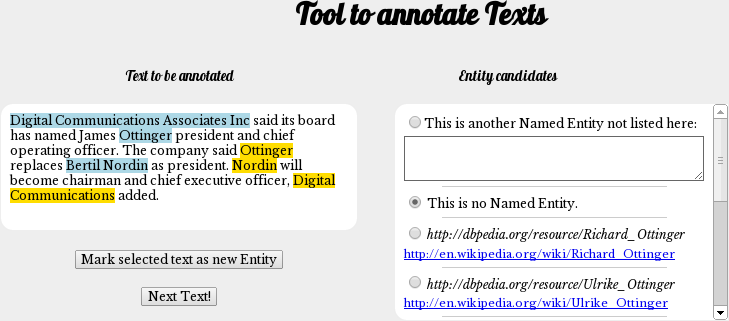
\includegraphics[width=\linewidth]{fig/qrtoolnew.png}
%    \caption{GUI of our annotation tool.}
%    \label{fig:qrtool}
%\end{figure*}

\subsection{Evaluation}
\label{results}



First, we evaluate AGDISTIS against AIDA and DBpedia Spotlight on three different knowledge bases using N3 corpora and the AIDA-YAGO2 corpus. 

AGDISTIS performs best on the \url{news.de} corpus, achieving a maximal 0.87 F\-measure for $\sigma = 0.71$ and $d = 2$ (see Table~\ref{tab:evalold}).
Our approach also outperforms the state of the art on Reuters-21578 corpus, see Figure~\ref{fig:reuters}, where it reaches 0.78 \mbox{F-measure} for $\sigma = 0.87$ and $d = 2$.
Considering the AIDA-YAGO2 dataset AGDISTIS achieves an \mbox{F-measure} of 0.73 for $\sigma = 0.89$ and $d = 2$.
%In combination with the results on RSS-500, 
Our results suggest that $d=2, \sigma=0.82$ and using DBpedia as \ac{KB} are a good setting for AGDISTIS and suffice to perform well. %The iteration of $\sigma$ between $0.7$ and $0.9$ can lead to an improvement of up to $6\%$ \mbox{F-measure}.
In the only case where $\sigma=0.29$ leads to better results (Reuters-21578 corpus), the setting $0.7<\sigma<0.9$ is only outperformed by 0.03 F-measure using YAGO as \ac{KB} for AGDISTIS.


\begin{table*}[htb!]
\centering

\resizebox{\textwidth}{!}{ 
\begin{tabular}{c ccc ccc c c}
\toprule
\textbf{Corpus}  & \multicolumn{6}{c}{\textbf{AGDISTIS}}	& \textbf{AIDA} & \textbf{Spotlight}\\\midrule
\textbf{$K$}& \multicolumn{3}{c}{{DBpedia}}& \multicolumn{3}{c}{{YAGO2}}	& {YAGO2} & {DBpedia}\\\midrule
				& \mbox{F-measure} 		& $\quad \sigma \quad $ & $\quad d \quad $ 	& \mbox{F-measure} & $\quad \sigma \quad $ & $\quad d \quad $ & \mbox{F-measure}  & \mbox{F-measure}\\
\cmidrule(r){2-4}  \cmidrule(r){5-7} \cmidrule{8-8} \cmidrule{9-9}
Reuters-21578	&  	\textbf{0.78}	&  			0.87		&  		2		& 	0.60	&  0.29		&  	3	&  	0.62		& 	0.56	\\
RSS-500 		&  	\textbf{0.75}	&  			0.76		&  		2		& 	0.53	&  0.82		&   2 	&  	0.60		& 	0.56	\\
\url{news.de} 	&  	\textbf{0.87}	&  			0.71		&  		2		& 	---		&   ---		&  ----	&  	----		& 	0.84	\\
AIDA-YAGO2	   	&  		0.73		&  			0.89		&  		2		& 	0.58	&  0.76		&   2 	&\textbf{0.83}	& 	0.57	\\
\bottomrule
\end{tabular}}
\caption{Evaluation of AGDISTIS against AIDA and DBpedia Spotlight. Bold indicates best \mbox{F-measure}.} \label{tab:evalold} 
\end{table*}
\begin{figure}[htb!]\centering
        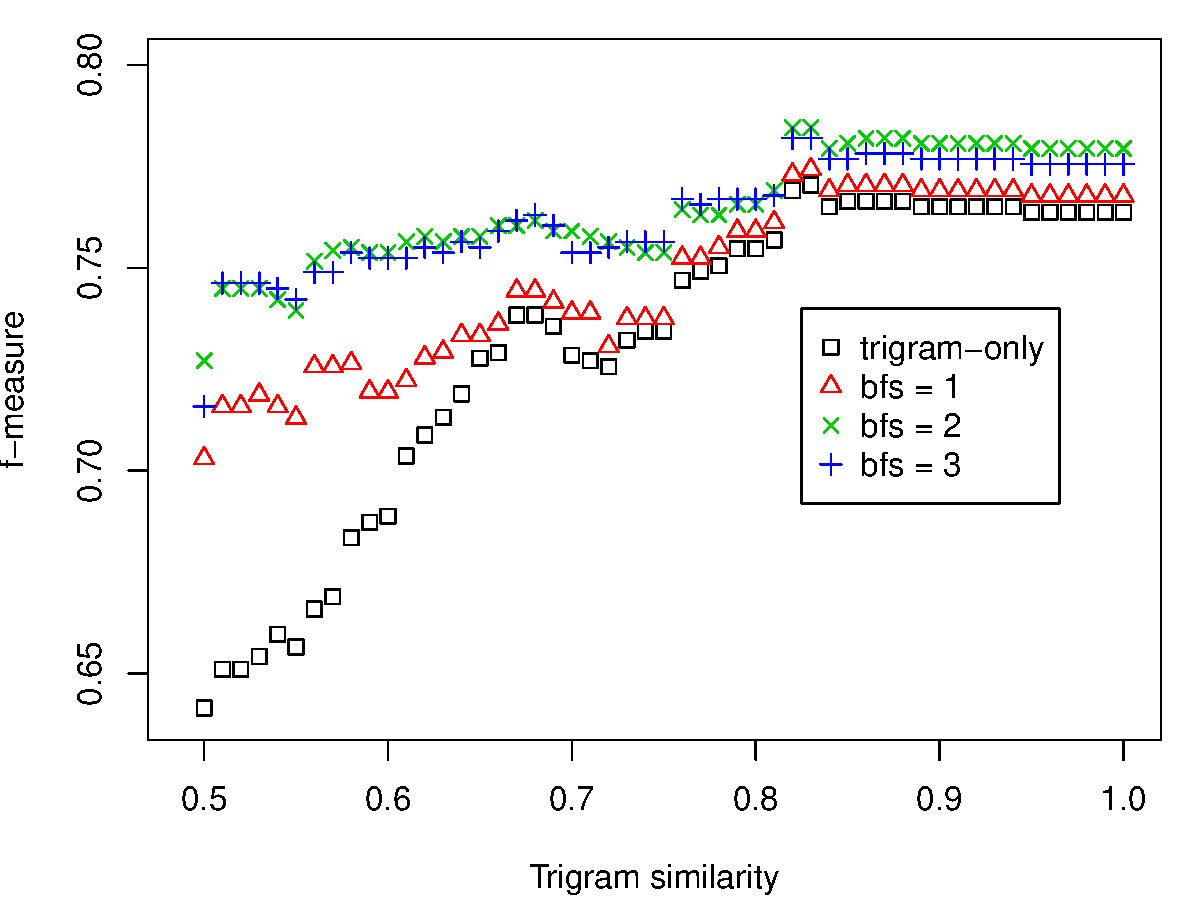
\includegraphics[width=0.9\linewidth]{part_02/unstructured_annotation/fig/reuters.pdf}
        %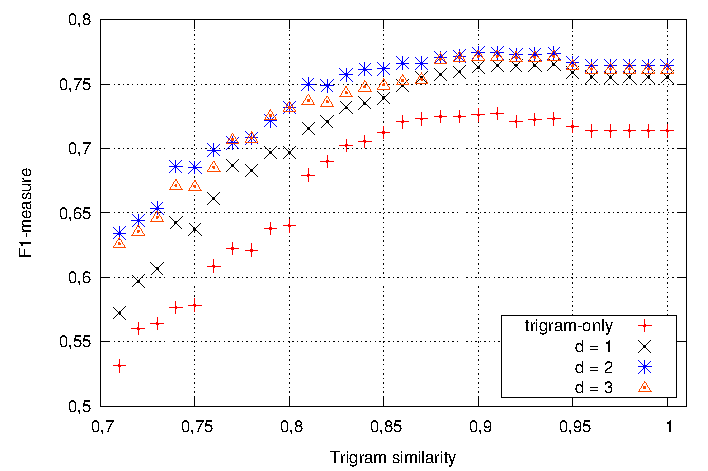
\includegraphics[width=0.9\linewidth]{fig/bfs_depth_diag.pdf}
    \caption{\mbox{F-measure} on the \textbf{Reuters-21578} corpus using DBpedia as \ac{KB}.}  \label{fig:reuters}
\end{figure}

Second, we compared our approach with TagMe 2 and DBpedia using datasets already implemented in the framework of Cornolti et al.
AGDISTIS has been setup to use a breadth-first search depth $d=2$ and a trigram similarity of $\sigma=0.82$.
All approaches used disambiguate w.r.t. the English DBpedia.
%TagMe 2 and DBpedia Spotlight are easily to test via web services while AIDA needs to be installed locally and run on a large machine. 
AIDA was ommitted from this evaluation because it has been shown to be outperformed by TagMe 2 in~\cite{cornolti} on the datasets we consider. 

AGDISTIS achieves \mbox{F-measures} between $0.31$ (IITB) and $0.76$ (MSNBC), see Table~\ref{tab:evalnew}.
We outperform the currently best disambiguation framework, TagMe 2, on three out of four datasets by up to $29.5\%$ F-measure. 
Our poor performance on IITB is due to AGDISTIS not yet implementing a paragraph-wise disambiguation policy. 
By now, AGDISTIS performs disambiguation on full documents.
The large number of resources in the IITB documents thus lead to our approach generating very large disambiguation graphs.
The explosion of errors within these graphs results in an overall poor disambiguation.
We will address this drawback in future work by fitting AGDISTIS with a preprocessor able to extract paragraphs from input texts.
The local vector-space model used by Spotlight performs best in this setting. 
\begin{table}[htb!]
    \centering

\begin{tabular}[tb]{@{}lllll@{}}
\toprule
Dataset                            & Approach          & \textbf{F1-measure}             & \textbf{Precision} & \textbf{Recall} \\ \midrule
\multirow{3}{*}{\begin{minipage}{0.8in}\textbf{AIDA/CO-NLL-TestB}\end{minipage}} & TagMe 2           & 0.565          & 0.58      & 0.551  \\
                                   & DBpedia Spotlight & 0.341          & 0.308     & 0.384  \\
                                   & AGDISTIS          & \textbf{0.596} & \textbf{0.642}     & \textbf{0.556}  \\ \midrule
\multirow{3}{*}{\textbf{AQUAINT}}  & TagMe 2           & 0.457          & 0.412     & \textbf{0.514}  \\
                                   & DBpedia Spotlight & 0.26           & 0.178     & 0.48   \\
                                   & AGDISTIS          & \textbf{0.547} & \textbf{0.777}     & 0.422  \\\midrule
\multirow{3}{*}{\textbf{IITB}}     & TagMe 2           & 0.408          & 0.416     & 0.4    \\
                                   & DBpedia Spotlight & \textbf{0.46}  & 0.434     & \textbf{0.489}  \\
                                   & AGDISTIS          & 0.31           & \textbf{0.646}     & 0.204  \\\midrule
\multirow{3}{*}{\textbf{MSNBC}}    & TagMe 2           & 0.466          & 0.431     & 0.508  \\
                                   & DBpedia Spotlight & 0.331          & 0.317     & 0.347  \\
                                   & AGDISTIS          & \textbf{0.761} & \textbf{0.796}     & \textbf{0.729}  \\ \bottomrule
\end{tabular}
\caption{Performance of AGDISTIS, DBpedia Spotlight and TagMe 2 on four different datasets using micro F-measure (\textbf{F1}).}
\label{tab:evalnew}
\end{table}
%\todo[inline]{Micha: the part "The iteration of $\sigma$ between $0.7$ and $0.9$ can lead to an improvement of up to $6\%$ \mbox{F-measure}" occurs two times. Remove one of them.}  



Delving deeper into AGDISTIS' results lead to the following insights:
\begin{itemize}
\item Varying the search depth $d$ does not significantly improve \mbox{F-measure} because within the underlying documents there are many similar named entities forming a shallow semantic background. However, using only string similarity measures ($d=0$) results in lower F-measure, see Figure \ref{fig:reuters}. % while the optimum has been found using $d=2$. %, see Figure~(\todo[inline]{here was a reference to a reuters figure}). 
\item The expansion policy can have considerable knock-on effects: Either the first entity and its expansions are disambiguated correctly or the wrong disambiguation of the first entity leads to an avalanche of false results in a loss of $\approx 4\%$ accuracy.
%\todo[inline]{Micha: Why accuracy while you always talk about F-measure?}
\item We observed a significant enhancement of AGDISTIS when adding surface forms to the labels of resources as explained in Section~\ref{choosing}.
Employing additional labels (such as surface forms gathered from Wikipedia) increased the \mbox{F-measure} of AGDISTIS by up to $4\%$. 
\item Using $n=1,2,4$ as n-gram similarity has been proven to perform worse than using trigram similarity,\,i.e., $n=3$.
Our results suggest that $d=2$ while using DBpedia as \ac{KB} is a good setting for AGDISTIS and suffice to perform well. 
The iteration of $\sigma$ between $0.7$ and $0.9$ can lead to an improvement of up to $6\%$ \mbox{F-measure} while $\sigma<0.7$ and $\sigma>0.9$ leads to a loss of F-measure.
\end{itemize}


Overall, our results suggest that $\sigma=0.82$ and $d=2$ is generally usable across datasets and knowledge bases leading to high quality results.\footnote{See also \url{http://139.18.2.164/rusbeck/agdistis/supplementary.pdf} and \url{http://139.18.2.164/rusbeck/agdistis/appendix.pdf}}
\todo[inline]{Appendix instead of footnotes}

%This is done by selecting all resources as candidates that are such that the similarity of at least one of its labels and the 
%The best similarity thresholds $\sigma$ w.r.t. disambiguation \mbox{F-measure} achieved by our approach were determined empirically iterating $\sigma$ between 0 and 1 in steps of 0.01. 
%Setting $\sigma=0.82$ turned out to be the best threshold independent of the analysed dataset.%\footnote{See our project side for further evaluation \url{http://aksw.org/Projects/AGDISTIS}}% (cf. Section~\ref{eval}).
%as shown in Figure~\ref{fig:influenceOfSurfaceForms}.
%This explains the worse results achieved by AGDISTIS when using YAGO2 as \ac{KB}. 

%\begin{figure}[htb!]\centering
%        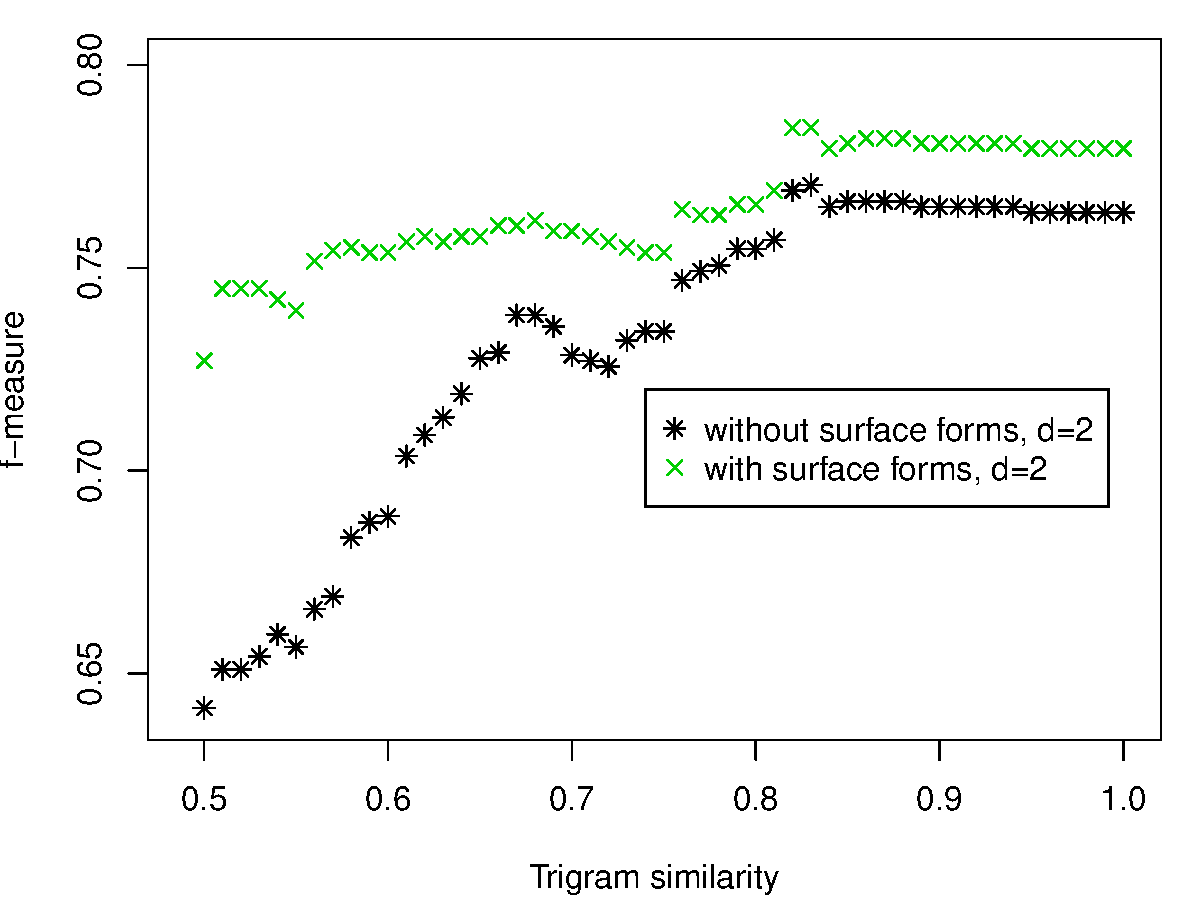
\includegraphics[width=0.9\linewidth]{fig/reutersWithoutSurfaceFormsAndBFS2.pdf}
        %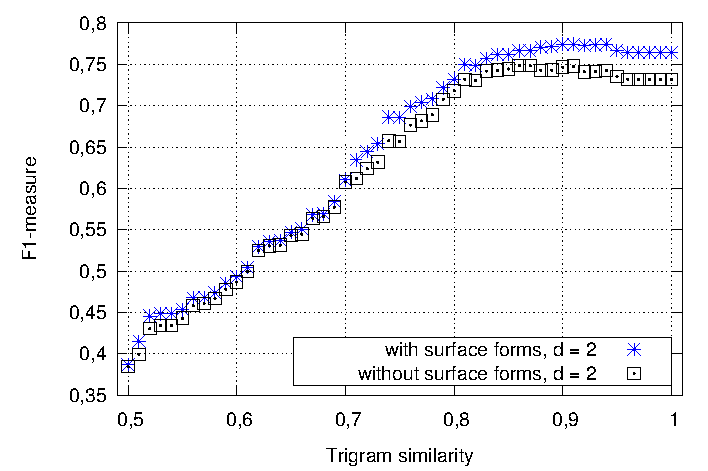
\includegraphics[width=0.9\linewidth]{fig/surface_forms_diag.pdf}
%    \caption{Influence of surface forms on the Reuters-21578 corpus and DBpedia as \ac{KB}.}\label{fig:influenceOfSurfaceForms}
%\end{figure}
%\todo[inline]{@axel: not using any graph just trigram sim is worse than the rest}
% for AGDISTIS are worse since our approach could not make use of surface forms as explained above. %, redirects or disambiguation entities, as explained above.
%Yet, given that a 1-1 mapping exists between YAGO2 and DBpedia URIs, we will consider the results of DBpedia for AGDISTIS in the following comparisons with other tools.
%\todo[inline}]{AN:Formally wrong. Either a 1-1 mapping exists or it does not}
%If there is no 1-1 mapping, the result of the disambiguation is counted as \emph{false positive}, which then results in low \mbox{F-measures} using YAGO2 as \ac{KB}.
%\todo{look at table caption please}


%\textbf{Comparison with AIDA.} 
%\todo[inline]{renew numbers}
%We compared our approach to AIDA by using the \textit{Cocktailparty configuration}\footnote{\url{https://github.com/yago-naga/aida}} (which is the recommended configuration for the framework) and applied the same restrictions that we used for AGDISTIS.
%The results of this evaluation on AIDA can be seen in Table~(\todo[inline]{here was a reference to the eval result}).
%Overall, AIDA performs well on arbitrary entities. 
%Yet, it is clearly outperformed by our approach on specific persons and organizations. 
%\todo[inline]{the statement above cant be seen in table 4, therefore we need to compare by type or clarify this sentence}
%In comparison to AIDA, AGDISTIS performs best on the Reuters-21578  where it surpasses AIDA by $\approx 0.16$ \mbox{F-measure}.
%Here AGDISTIS benefits from surface forms and its expansion policy.
%Furthermore, AGDISTIS outperforms AIDA with the RSS-500 corpus by $\approx 0.15$ \mbox{F-measure}.
%This corpus differs considerably from the Reuters-21578 corpus due to the small disambiguation contexts and graphs evolving from two named entities per text only.
%Note that AGDISTIS also outperforms AIDA for our overall default setting of $\sigma = 0.81$, apart from the result on the AIDA-YAGO2 corpus.
%AIDA could not be run on the \url{news.de} corpus as it can only deal with English.
%Here, the \emph{language-independence} of AGDISTIS provides a significant improvement of the state of the art.
%AIDA performs better on AIDA-YAGO2 achieving an \mbox{F-measure} of 0.83 due to the large contexts of the documents (see Table~(\todo[inline]{here was a reference to a data table})).
%This is clearly due to AGDISTIS being tuned towards smaller contexts since these are more common in WND, see Table~(\todo[inline]{here was a reference to a data table}).
%In particular, the AIDA-YAGO2 corpus contains many sport teams from cities and countries like \texttt{Barcelona} where AGDISTIS identifies \texttt{dbr:Barcelona} and \texttt{dbr:FC\_Barcelona} as resources. Since \texttt{dbr:Barcelona} has a higher authoritative score than \texttt{dbr:FC\_Barcelona}, AGDISTIS' disambiguation results in a \emph{false positive} in this particular case.
%As shown in Table~\ref{eval} using YAGO2 leads to worse results since AGDISTIS (in contrast to AIDA) does not possess surface forms for YAGO2.
%\todo[inline]{No appendiy, how to solve this?}

%\textbf{Comparison with DBpedia Spotlight.}
%\todo[inline]{renew the numbers}
%In order to compare DBpedia Spotlight with AGDISTIS Cornolti et al.~\cite{cornolti} used Spotlight's Web services.\footnote{\url{https://github.com/dbpedia-spotlight/dbpedia-spotlight/wiki/Web-service}}

%The results of the evaluation are shown in Table~\ref{tab:eval}.
%Spotlight performs best on the \url{news.de} dataset (\mbox{F-measure} = 0.84) and worst on the Reuters-21578 dataset (\mbox{F-measure} = 0.56), Table~(\todo[inline]{here was a reference to the eval result}).
%This is possibly due to the datasets age of over 20 years and missing historic data in DBpedia.
%When evaluated against the AIDA-YAGO2 corpus Spotlight achieves a \mbox{F-measure} of 0.57.
%Using the RSS-500 dataset Spotlight is only able to generate a \mbox{F-measure} of 0.56.
%\todo[inline]{renew the number}
%AGDISTIS outperforms Spotlight by at least $\approx 0.15$ \mbox{F-measure}. % using DBpedia as \ac{KB}. on each English dataset.

%AGDISTIS performs better on two of the datasets and is even usable for the German dataset as it is agnostic towards the language of the used \ac{KB}.
%As can be seen in Figure \ref{fig:relation} the number of entities per text is an important criteria for disambiguation.

%\textbf{Run time analysis.}
%On average AGDISTIS is more time-efficient than AIDA with respect to the best %corresponding configuration.
%While AGDISTIS finished its computation on Reuters-21578 corpus in 549\,seconds (s), AIDA needed more than twice as much time,\,i.e., 1,296\,s.
%This behavior can also be seen on the short documents of the RSS-500 dataset, where AIDA needed 4,919\,s and our approach only 623\,s.
%Moreover, AGDISTIS outperforms AIDA with 3,946\,s to 51,435\,s run time on the AIDA-YAGO2 corpus.
%\todo[inline]{is not comparable anymore since we needed to run it in the cloud}
%Details can be found on the project website.



%\subsection{English and German Evaluation.} AGDISTIS has been evaluated on 9 different datasets from diverse domains such as news, sports or buisiness reports.
%For English datasets AGDISTIS is able to outperform the currently best disambiguation framework, TagMe2, on three out of four datasets by up to 29.5\% F-measure. 
%Considering the only German dataset available for named entity disambiguation, i.e., \url{news.de}~\cite{n3}, we are able to outperform the only competitor DBpedia Spotlight by 3\% F-measure.

%\subsection{How the Chinese version was generated}



%However, the latest available Linked Data --- DBpedia 3.9 --- has no such information for Chinese. 
%Therefore, we created triples containing \texttt{\ac{RDF}:type} as predicate by translating the English ones to Chinese. 
%Specifically, we use inter-language links extracted by DBpedia 
%\footnote{Available from \url{http://wiki.dbpedia.org/Downloads39\#inter-language-links}}, in which a English resource is represented in different other languages. 
%An English-Chinese pair of phrases for each resource is extracted using the following regular expression\footnote{{\it zh} is the language code for Chinese.}:
%\begin{verbatim}
%``$\langle http://dbpedia\backslash.org/resource/(.*)\rangle\backslash s*\langle.*\rangle \backslash s*\langle http://zh.dbpedia.org/resource/(.*)\rangle\backslash s*.$"
%\end{verbatim}
%, resulting a phrase table with 420,047 English-Chinese pairs.

%For each \ac{RDF}:type triple in the English DBpedia, if the name of the subject appears in the phrase table, it is mapped to Chinese according to the phrase table. In this way, a total of 1,234,783 triples are extrated for Chinese.

%Both the data stored in a Lucene 4.5.1 Index and the phrase table can be found at \url{http://139.18.2.164/rusbeck/}.

%\subsection{Accuracy results of the Chinese version}
%In this section, we will introduce a new Chinese benchmark and the evaluation results.

\subsection{Chinese Benchmark}
\label{sec:chinese}
The key to extend AGDISTIS to support a new language, in this case Chinese, is to provide the needed \ac{RDF} data for this particular language, especially \texttt{rdf:type} information. 
To evaluate the Chinese version of AGDISTIS, a Chinese benchmark has been created in the context of \ac{QA}.
The disambiguation of named entities is a key step to answer natural language questions based on Linked Data. 
%\subsubsection{Results}

%\noindent \textbf{Chinese Evaluation.} We evaluated the Chinese version of AGDISTIS within a question answering setting. 
To this end, we used the multilingual benchmark provided in QALD~4~\cite{qald4}. 
Since the Chinese language is not supported, we extended the QALD~4 benchmark by translating the English questions to Chinese and inserted the named entity links manually.
%The accuracies achieved by AGDISTIS for the train and test datasets are 65\% and 70\% respectively. 
%We also performed a fully automatic evaluation by using the Chinese segmentation and named-entity recognition algorithms provided by LTP-Cloud\footnote{\url{http://www.ltp-cloud.com/}}. 
%The accuracies sank to 32\% and 38\%.
%These results indicate the need for better resources for Entity Recognition in Chinese.

We first report the disambiguation accuracies by assuming the named entities are given. It allows a fair comparison to other disambiguation algorithms because named entity disambiguation performance is highly depended on named-entity recognition results. The accuracy is measured at a sentence level by assuming a correct disambiguation should recognize and link all the entities in a sentence, which is essential for further steps in question answering. The accuracies for the training and testing are 65\% and 70\% respectively. 

%We also performance a fully automatic evaluation by using the Chinese segmentation and named-entity recognition algorithms provided by LTP-Cloud\footnote{\url{http://www.ltp-cloud.com/}}. 
%The accuracies are 32\% and 38\%.


 
\section{Demonstration}
%\begin{itemize}
%\item Moreover, the output format of AGDISTIS will be explained. 
%An online version of the demo is available at \url{http://agdistis.aksw.org/demo}.
%The aim of this demo is to present the English, German and Chinese version of our framework based on DBpedia.
%\item A demo of our approach (integrated into the Named Entity Recognition framework FOX~\cite{FOX}) can be found at \url{http://fox.aksw.org}. 
%\item In this demo, we will present AGDISTIS deployed on three different languages (English, German and Chinese) and three different knowledge bases (DBpedia, the German DBpedia and the Chinese DBpedia).
%To the best of our knowledge, we therewith provide the first Chinese instantiation of entity linking to DBpedia.
%\item We will also demonstrate the AGDISTIS web services endpoints for German, English and Chinese disambiguation and show how data can be sent to the endpoints.
%\item Moreover, the output format of AGDISTIS will be explained.
%
%\end{itemize}

Within our demonstration, we aim to show how AGDISTIS can be used by non-expert as well as expert users. \footnote{An online version of the demo is available at \url{http://agdistis.aksw.org/demo}.}
Another aim of this demo is to present the English, German and Chinese version of our framework based on DBpedia.
For non-experts, we provide a graphical user interface (GUI).
Experts can choose to use the REST interfaces provided by the tool. % or use a Java snippet to call the REST interface.
The whole of this functionality, which will be described in more details in the following. % sections, will also be demonstrated at the conference.

\subsection{AGDISTIS for non-expert users}
A screenshot of the AGDISTIS GUI is shown in Figure~\ref{fig:gui}.
This GUI supports the following workflow.

\begin{figure}[htb!]
\centering
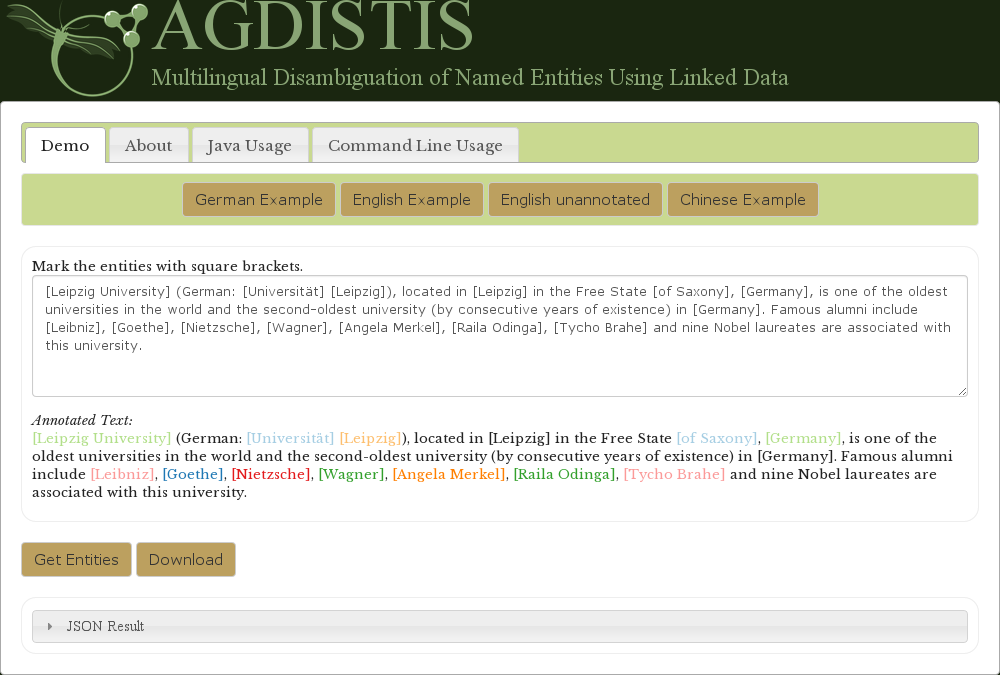
\includegraphics[width=\textwidth]{part_02/unstructured_annotation/fig/GUI.png}
\caption{Screenshot of the demo with an English example which is already annotated.}
\label{fig:gui}
\end{figure}

\noindent\textbf{Entity Recognition}
After typing or pasting text into the input field, users can choose between either annotating the entities manually or having the entities detected automatically.
In the first case, the labels of the entities are to be marked by using square brackets, see central panel of Figure~\ref{fig:gui}.
In the case of an automatic annotation, we send the text to the FOX framework, which has been shown to outperform the state of the art in~\cite{FOX}.
%In our current implemen
%Since there is no multilingual \ac{NER} tool available, an automatic annotation of entities works only for English texts.
%We will demonstrate this feature by using both manually pre-annotated text and text without annotations in our examples (see upper bar of Figure~\ref{fig:gui}).
%Moreover, we will allow the crowd to enter arbitrary texts that pertain to their domain of interest.

\noindent\textbf{Automatic Language Detection}
Once the user has set which entities are to be disambiguated, the marked-up text is sent to the language detection module based on~\cite{nakatani2010langdetect}.
We chose this library because it is both precise ($>99\%$ precision) and time-efficient.
If the input is detected to belong to one of the languages we support (i.e., German, Chinese, English), then we forward the input to a dedicated AGDISTIS instance for this given language.
In all other cases, an error message is shown to the user, pointing towards the language at hand not being supported.
The main advantage of this approach is that the user does not need to select the language in which the text is explicated manually, thus leading to an improved user experience. 
%We will demonstrate this feature by entering text in different languages (German, English, French, Chinese, etc.) and presenting the output of the framework for each of these test cases.

\noindent\textbf{Entity Linking} 
This is the most important step of the whole workflow.
The annotated text is forwarded to the corresponding language-specific deployment of AGDISTIS, of which each relies currently on a language-specific version of DBpedia 2014. 
%The approach underlying AGDISTIS~\cite{agdistis_iswc} is language-independent and combines breadth-first search and the well-known  \ac{HITS} algorithm. 
%In addition, string similarity measures and label expansion heuristics are used to account for typos and morphological variations in naming.
%Moreover, Wikipedia-specific surface forms for resources can be used. 

\noindent\textbf{Output}
Within the demo the annotated text is shown below the input field where disambiguated entities are colored to highlight them. 
While hovering a highlighted entity the disambiguated URI is shown.
We will demonstrate the output of the entity linking by using the examples shown in the upper part of Figure~\ref{fig:gui}. 
The output of the system will be shown both in a HTML version and made available as a download in JSON. 
%Moreover, we will allow interested participants to enter their own examples and view the output of the tool.

\subsection{AGDISTIS for expert users}

%To support different languages, we set up a REST URI for each of the language versions.
%those\footnote{\url{http://139.18.2.164:8080/AGDISTIS_DE}}\footnote{\url{http://139.18.2.164:8080/AGDISTIS_ZH}}\footnote{\url{http://139.18.2.164:8080/AGDISTIS}}.
Each of these endpoints understands two mandatory parameters: (1) \texttt{text} which is an UTF-8 and URL encoded string with entities annotated with XML-tag \texttt{<entity>} and (2) \texttt{type='agdistis'} to disambiguate with the AGDISTIS algorithm.
In the future, several wrappers will be implemented to use different entity linking algorithms for comparison.
Following, a CURL\footnote{\url{http://curl.haxx.se/}} snippet shows how to address the web service, see also \url{http://agdistis.aksw.org}:
\begin{verbatim}
curl --data-urlencode "text='<entity>Barack Obama</entity> arrives 
in <entity>Washington, D.C.</entity>.'" -d type='agdistis' 
{AGDISTIS URL}/AGDISTIS
\end{verbatim}


%architecture, what are the main steps
%GOAL is to provide entity linking results to several languages which are show on the website and downloadable as JSON
%1 we will present and explain how AGDISTIS works and how multilinguality is achieved
%2 Users can try different inputs at the demo station and tell us, what quality they expect and which languages they want
%3 finally we will show how the results can be downloaded or seen online and how the annotation of more or less entities changes the behaviour of AGDISTIS
%benchmarks will be shown as well and people will be invited to use our for free endpoint for their projects so we can store the use case data and improve our approach similar to the feedback API of spotlight and fox


\section{Conclusion \& Contributions}
\label{sec:conclusion}
%\todo[inline]{Micha: AIDA is missing in the conclusion.}
We presented AGDISTIS, a novel named entity disambiguation that combines the scalable \ac{HITS} algorithm and breadth-first search with linguistic heuristics.
Our approach outperforms the state-of-the-art algorithms TagMe 2, AIDA and DBpedia Spotlight while remaining quadratic in its time complexity. 
Moreover, our evaluation suggests that while the approach performs well in and of itself, it can benefit from being presented with more linguistic information such as surface forms. 
We presented the demo of AGDISTIS for three different languages on three different DBpedia-based knowledge bases.
Further, we created the first \ac{NED} system for the Chinese language based on Linked Data.
%Furthermore, we measured the effect of evolving the structure of the underlying knowledge base.
%We observed the significance of properties on the \mbox{F-measure} performance of our system.
%Our results suggest that only a few \ac{RDF} properties contribute significantly to enhancing the performance of AGDISTIS.

We see this work as the first step in a larger research agenda.
Based on AGDISTIS, we aim to develop a new paradigm for realizing \ac{NLP} services which employ community-generated, multilingual and evolving Linked Open Data background knowledge.
Other than most work, which mainly uses statistics and heuristics, we aim to truly exploit the graph structure and semantics of the background knowledge.

Since AGDISTIS is agnostic of the underlying \ac{KB} and language-independent, it can profit from growing \ac{KB}s as well as multilingual Linked Data.
In the future, we will thus extend AGDISTIS by using different underlying \ac{KB}s and even more domain-specific datasets.
%An evaluation of Babelfy against our approach will be published on the project website.
Moreover, we will implement a sliding-window-based extension of AGDISTIS to account for large amounts of entities per document.
%A novel avenue of research would be combining AGDISTIS with topic modelling~\cite{Blei:2003:LDA:944919.944937}. Preliminary experiments in this direction show that we can improve the F-measure of our approach by at least 1\% on all datasets.
%In the future we intend to look for larger, more domain-specific and even more insightful disambiguation datasets to refine and test AGDISTIS.
%Moreover, a deeper evaluation of ontology structures towards disambiguation accuracies is needed.
%Answering those research questions will expose possible performance-enhancing extensions.
%


%In future work, we aim to create a single-server multilingual version of the framework that will intrinsically support several languages at the same time.
%To this end, we will use a graph merging algorithm to combine the different versions of DBpedia to a single graph.
%The disambiguation steps will then be carried out on this unique graph.
%expand different knowledge base and 
%a full dbpedia supported multilingual version

AGDISTIS is integrated into FOX~\cite{FOX}, an ensemble learning based \ac{NER}~framework which can be found at \url{http://fox.aksw.org}. 
Furthermore, AGDISTIS is integrated in to the entity evaluation platform GERBIL~\cite{GERBIL}, see \url{http://gerbil.aksw.org/gerbil/}.
\todo[inline]{@Axel: Aufrufzahlen nennen?}
